\chapter{Background}\label{ch:background}


\section{Cryptography Primitives}\label{sec:cryptography}

\subsection{Hash Functions}\label{subsec:crypto:hash}

Hash functions are cryptographic functions designed to behave like random
functions~\cite{smart2016randomOracleModel}.
When building a security proof, they can be assumed to have the following properties~\cite{smart2016randomOracleModel,
    smart2016hashFunctions}:
% FIXME needs references
\begin{description}
    \item[Determinism] A hash function always produces the same output for the same input
    \item[One-way] It is computationally impossible to compute the preimage for some output of a hash function
    \item[Uniformity] Outputs of a hash function are expected to be uniformly distributed.
    In practice, the output space of a hash function is finite, so \textit{collisions} (where two inputs produce the
    same output) are possible, but uniformity ensures this is an unlikely scenario.
\end{description}

\subsection{Public Key Cryptography}\label{subsec:crypto:pubkey}

In public key cryptography, two communicating parties (say Alice and Bob) can communicate privately by using pairs of
numbers that are related mathematically and which allow converting cleartext into cyphertext and
back~\cite{smart2016publicKey}.
This pair of numbers is called an asymmetric keypair, and is composed of a \textbf{public key} $e$ and a \textbf{private
key} $d$.\\

In this example, if Alice wishes to communicate with Bob, Bob can generate a keypair $(d, e)$ and publish $e$.
Alice can then encrypt her cleartext with $e$, and only Bob will be able to decrypt it (because only Bob knows $d$).

\begin{figure}[th]
    \centering
    \tikzset{every picture/.style={line width=0.75pt}} %set default line width to 0.75pt
    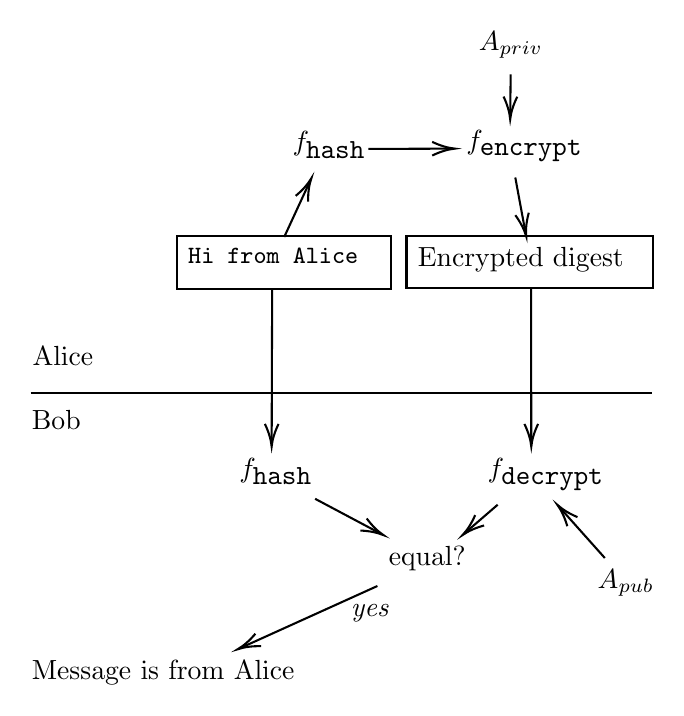
\begin{tikzpicture}[x=0.75pt,y=0.75pt,yscale=-1,xscale=1]
%uncomment if require: \path (0,355); %set diagram left start at 0, and has height of 355

%Straight Lines [id:da017592532205451983]
        \draw    (60.54,179.69) -- (359.87,179.69) ;

% Text Node
        \draw    (131,104) -- (234,104) -- (234,129.67) -- (131,129.67) -- cycle ;
        \draw (135,108.67) node [anchor=north west][inner sep=0.75pt]   [align=left] {\small \texttt{Hi from Alice}};
% Text Node
        \draw (185.33,52.33) node [anchor=north west][inner sep=0.75pt]   [align=left] {$\displaystyle f_{\texttt{hash}}$};
% Text Node
        \draw (275,4.33) node [anchor=north west][inner sep=0.75pt]   [align=left] {$\displaystyle A_{priv}$};
% Text Node
        \draw (332.33,263.33) node [anchor=north west][inner sep=0.75pt]   [align=left] {$\displaystyle A_{pub}$};
% Text Node
        \draw (269,52) node [anchor=north west][inner sep=0.75pt]   [align=left] {$\displaystyle f_{\texttt{encrypt}}$};
% Text Node
        \draw    (241.67,104) -- (360.67,104) -- (360.67,129.33) -- (241.67,129.33) -- cycle ;
        \draw (245.67,108.33) node [anchor=north west][inner sep=0.75pt]   [align=left] {Encrypted digest};
% Text Node
        \draw (60,156) node [anchor=north west][inner sep=0.75pt]   [align=left] {Alice};
% Text Node
        \draw (59.67,186.67) node [anchor=north west][inner sep=0.75pt]   [align=left] {Bob};
% Text Node
        \draw (159.67,209.67) node [anchor=north west][inner sep=0.75pt]   [align=left] {$\displaystyle f_{\texttt{hash}}$};
% Text Node
        \draw (279.33,209.67) node [anchor=north west][inner sep=0.75pt]   [align=left] {$\displaystyle f_{\texttt{decrypt}}$};
% Text Node
        \draw (231.67,252.33) node [anchor=north west][inner sep=0.75pt]   [align=left] {equal?};
% Text Node
        \draw (59.67,307.33) node [anchor=north west][inner sep=0.75pt]   [align=left] {Message is from Alice};
% Text Node
        \draw (208.67,280.33) node [anchor=north west][inner sep=0.75pt]   [align=left] {\textit{{ yes}}};
% Connection
        \draw    (182.78,104.67) -- (195.03,78.15) ;
        \draw [shift={(195.87,76.33)}, rotate = 114.8] [color={rgb, 255:red, 0; green, 0; blue, 0 }  ][line width=0.75]    (10.93,-3.29) .. controls (6.95,-1.4) and (3.31,-0.3) .. (0,0) .. controls (3.31,0.3) and (6.95,1.4) .. (10.93,3.29)   ;
% Connection
        \draw    (223.33,62.25) -- (263,62.11) ;
        \draw [shift={(265,62.1)}, rotate = 179.79] [color={rgb, 255:red, 0; green, 0; blue, 0 }  ][line width=0.75]    (10.93,-3.29) .. controls (6.95,-1.4) and (3.31,-0.3) .. (0,0) .. controls (3.31,0.3) and (6.95,1.4) .. (10.93,3.29)   ;
% Connection
        \draw    (294.1,76) -- (298.98,102.37) ;
        \draw [shift={(299.35,104.33)}, rotate = 259.5] [color={rgb, 255:red, 0; green, 0; blue, 0 }  ][line width=0.75]    (10.93,-3.29) .. controls (6.95,-1.4) and (3.31,-0.3) .. (0,0) .. controls (3.31,0.3) and (6.95,1.4) .. (10.93,3.29)   ;
% Connection
        \draw    (291.87,26.33) -- (291.66,46) ;
        \draw [shift={(291.64,48)}, rotate = 270.59] [color={rgb, 255:red, 0; green, 0; blue, 0 }  ][line width=0.75]    (10.93,-3.29) .. controls (6.95,-1.4) and (3.31,-0.3) .. (0,0) .. controls (3.31,0.3) and (6.95,1.4) .. (10.93,3.29)   ;
% Connection
        \draw    (176.96,129.67) -- (176.72,203.67) ;
        \draw [shift={(176.71,205.67)}, rotate = 270.19] [color={rgb, 255:red, 0; green, 0; blue, 0 }  ][line width=0.75]    (10.93,-3.29) .. controls (6.95,-1.4) and (3.31,-0.3) .. (0,0) .. controls (3.31,0.3) and (6.95,1.4) .. (10.93,3.29)   ;
% Connection
        \draw    (301.69,129.33) -- (301.81,203.67) ;
        \draw [shift={(301.81,205.67)}, rotate = 269.91] [color={rgb, 255:red, 0; green, 0; blue, 0 }  ][line width=0.75]    (10.93,-3.29) .. controls (6.95,-1.4) and (3.31,-0.3) .. (0,0) .. controls (3.31,0.3) and (6.95,1.4) .. (10.93,3.29)   ;
% Connection
        \draw    (197.67,230.82) -- (228.87,247.4) ;
        \draw [shift={(230.63,248.33)}, rotate = 207.98] [color={rgb, 255:red, 0; green, 0; blue, 0 }  ][line width=0.75]    (10.93,-3.29) .. controls (6.95,-1.4) and (3.31,-0.3) .. (0,0) .. controls (3.31,0.3) and (6.95,1.4) .. (10.93,3.29)   ;
% Connection
        \draw    (285.62,233.67) -- (270.15,247.03) ;
        \draw [shift={(268.64,248.33)}, rotate = 319.18] [color={rgb, 255:red, 0; green, 0; blue, 0 }  ][line width=0.75]    (10.93,-3.29) .. controls (6.95,-1.4) and (3.31,-0.3) .. (0,0) .. controls (3.31,0.3) and (6.95,1.4) .. (10.93,3.29)   ;
% Connection
        \draw    (227.67,272.83) -- (162.1,302.51) ;
        \draw [shift={(160.28,303.33)}, rotate = 335.64] [color={rgb, 255:red, 0; green, 0; blue, 0 }  ][line width=0.75]    (10.93,-3.29) .. controls (6.95,-1.4) and (3.31,-0.3) .. (0,0) .. controls (3.31,0.3) and (6.95,1.4) .. (10.93,3.29)   ;
% Connection
        \draw    (337.23,259.33) -- (315.66,235.16) ;
        \draw [shift={(314.33,233.67)}, rotate = 48.25] [color={rgb, 255:red, 0; green, 0; blue, 0 }  ][line width=0.75]    (10.93,-3.29) .. controls (6.95,-1.4) and (3.31,-0.3) .. (0,0) .. controls (3.31,0.3) and (6.95,1.4) .. (10.93,3.29)   ;

    \end{tikzpicture}
    \decoRule
    \caption[Asymmetric signing scheme]{An asymmetric key signing scheme where Bob is able to verify only Alice could
    have written '\texttt{Hi from Alice}'}
    \label{fig:pubkey-signing}
\end{figure}

Conversely, the same keypair can be used by Bob to send a message to Alice where Alice can verify that only Bob
could have written the message.
This is called \textit{signing}~\cite{smart2016signatures} and, more generally, it allows a sender of a message to
prove they are the authors of the message to a recipient.
An example of a signing scheme can be seen in Figure~\ref{fig:pubkey-signing}.

\subsection{Secure Digital Timestamps}\label{subsec:crypto:timestamps}
% TODO citation for definiton
\textit{Trusted (digital) timestamping} is the process of securely proving that a document (for our purposes, a blob of
bytes) was created, was modified at, or existed at a certain point in time.
% TODO citation for widely used
In industry this is commonly implemented by trusting a Time Stamping Authority (TSA)~\cite{timestamps_tsp_rfc} that
signs (see~\nameref{subsec:crypto:pubkey}) a concatenation of the hash of the document and a timestamp representing some
time $t$.
Therefore a party that trusts the TSA to provide the right timestamp can verify that, when the TSA made the signature,
the current time was $t$.
\\

This method can be used for confidential data because the TSA does not perform the hashing of the original document
themselves - they are exposed only to its digest.

Additionally, the requester of the timestamp cannot deny they were not in possession of the original data at the time
% TODO verify statement
$t$ given by the timestamp, because it was them that produced its hash digest.

\subsubsection{Decentralised Timestamps}

Secure timestamps can also be achieved without relying on trusted parties by publishing the document digest to a
blockchain~\cite{gipp2015timestamps_btc}: blocks are public and cannot be tampered with (see~\nameref{subsec:btc:pow}),
so putting a signed digest in a block shows that the signer knew the original document at the time the block was
accepted by the network.


\section{Bitcoin Protocol}\label{sec:bitcoin}

Blockchain technology was introduced in~\cite{nakamoto2008bitcoin} as a decentralised system allowing for electronic
cash payments.
Blockchains are immutable distributed ledgers where participants' balances can be verified by every other participant,
and it is computationally hard to tamper with balances to perform attacks (such as performing a transaction where a
participant spends more funds than what they own).

I will provide a brief overview of how Bitcoin provides these guarantees.

\subsection{Transactions}\label{subsec:btc:txs}

\cite{nakamoto2008bitcoin} defines an \textit{electronic coin} as a chain of signatures: a payer can use their private
key, the hash of the previous transaction, and the payee's public key to create a signed hash that can be verified by
the payee (and used by them for \textit{their} next transaction).
This is illustrated in Figure~\ref{fig:bitcoin-tx}.

\begin{figure}[th]
    \centering
    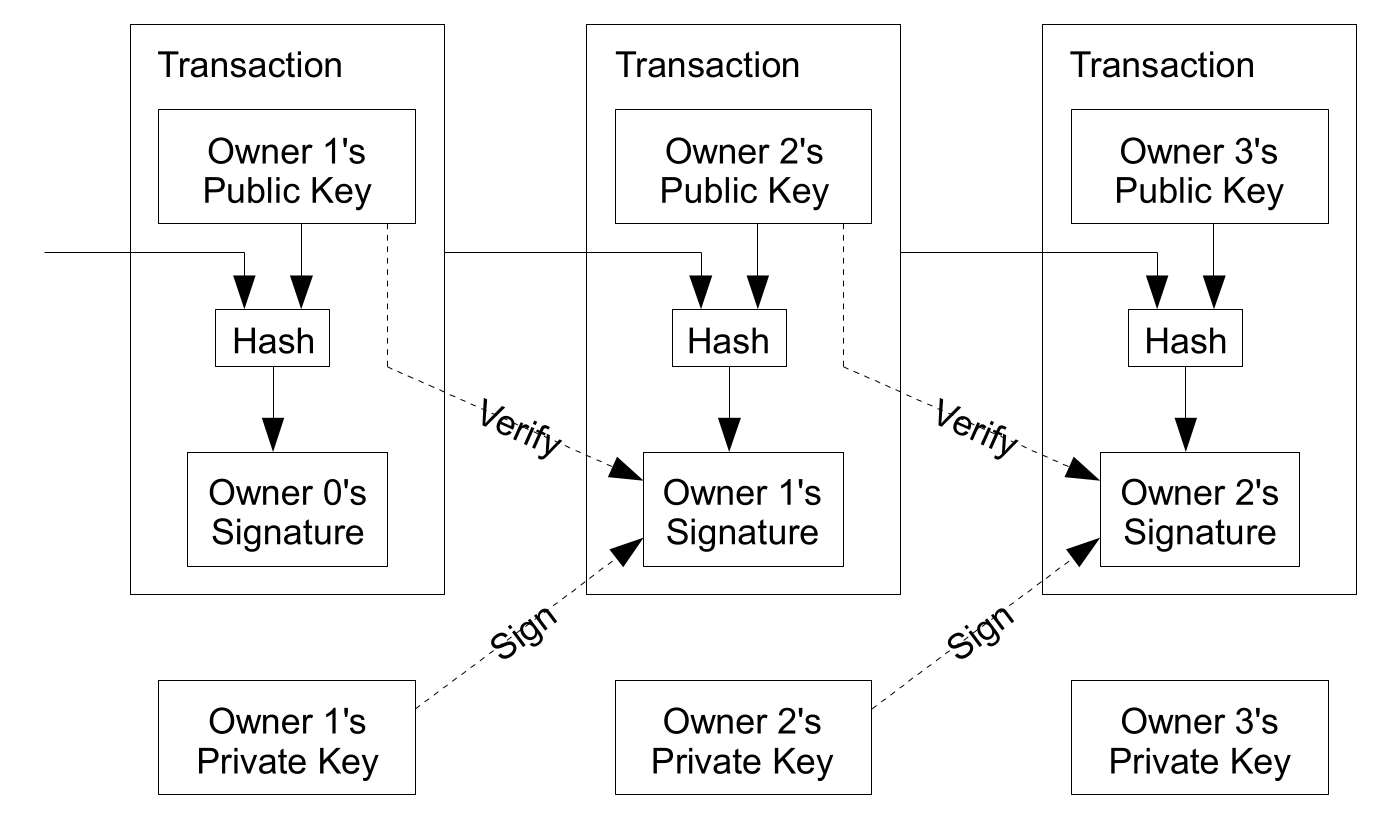
\includegraphics[width=0.8\columnwidth]{figures/bitcoin-tx}
    \caption[Bitcoin coin ownership transfer]{Transfer of ownership signature chain, from~\cite{nakamoto2008bitcoin}}
    \label{fig:bitcoin-tx}
\end{figure}

This ensures that, as long as a participants sign transactions at most once:
\begin{itemize}
    \item By verifying the chain of signatures, every participant can verify which participant owns which coin
    \item Only the owner of a coin can initiate a transaction with that coin
\end{itemize}

Bitcoin enforces that participants can only sign transactions once thanks to its proof-of-work
(see~\ref{subsec:btc:pow}) algorithm.

\subsection{Proof-Of-Work}\label{subsec:btc:pow}

Bitcoin ensures 'unique signatures' in transactions by grouping transactions in immutable, public \textit{blocks}.
Participants can then verify a payer has not signed a hash of a single transaction twice by looking at all existing
transactions.\\

Blocks are made immutable by including in them a value (called a \textit{nonce}) and the hash of the previous block.
% TODO verify it is the hash of the entire block that must yield the zeroes (implementation detail really)
The protocol then accepts only blocks where the $n$ first bits of its hash are zeroes. \\

Thus, in order to publish a block a participant must do work to find a nonce such that the block's hash meets this
condition - then other participants can verify its validity with a single hash operation.
This guarantees that a block cannot be changed (ie, a new copy published) without redoing the computational work.
Because blocks are chained (they include the hash of the previous block), in order to modify a transaction in the past
an adversary needs to redo the computational work for every block since that transaction (see Figure
\ref{fig:bitcoin-blockchain}).
% TODO implementation of mining rewards
Additionally, participants that successfully find a suitable nonce and propose new blocks (also referred to as
\textit{miners}) are allowed to add a specific transaction to the block where they own a newly created coin (also
referred to as \textit{mining reward}).

\begin{figure}[th]
    \centering
    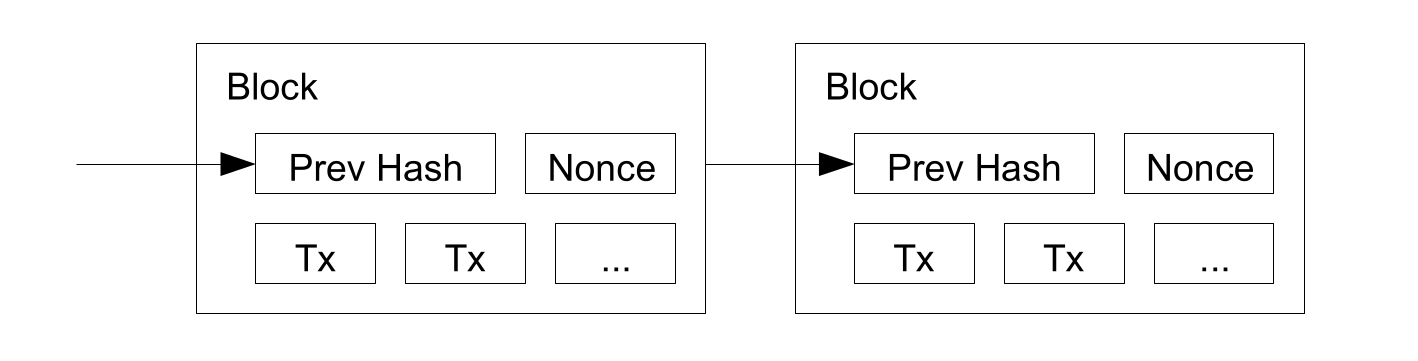
\includegraphics[width=0.8\columnwidth]{figures/bitcoin-blockchain}
    \caption[Two last blocks in a blockhain]{Two last blocks in a blockchain, from~\cite{nakamoto2008bitcoin}}
    \label{fig:bitcoin-blockchain}
\end{figure}

This model of consensus ensures that
\begin{itemize}
    \item Participants have a monetary incentive to stay honest with respect to the protocol
    \item An honest chain will out-compete an adversary's chain as long as the majority of computing power is honest
\end{itemize}

\subsection{Further details of the Bitcoin protocol}\label{subsec:btc.details}
\begin{figure}[th]
    \centering
    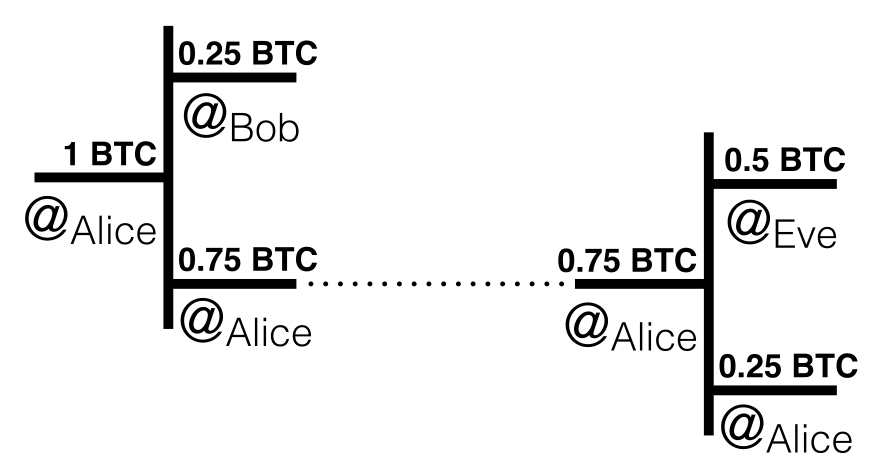
\includegraphics[width=0.6\columnwidth]{figures/bitcoin-2txs-outputs}
    \caption[Outputs and Inputs of two consecutive Transactions]{The outputs of a transaction correspond to
    the input of the next transaction (miner's fee not represented) from~\cite{gervais2022distribLedgers_transactionsInBitcoin}}
    \label{fig:bitcoin-2txs-outputs}
\end{figure}

While I provide a high-level overview of what makes the protocol function, there are many more details that combined
allow for more efficiency and usability:
\begin{itemize}
    \item Transactions may have several inputs and outputs, so participants can transfer amounts rather than single
    \textit{electronic coins}.
    When performing a payment, a typical transaction by Alice has two outputs: the amount she is paying Bob and the
    remainder, which makes up the rest of her funds (see Figure~\ref{fig:bitcoin-2txs-outputs}).
    Thus, a participant's balance is the sum of all the unspent outputs of previous transactions (the set of unspent
    outputs is commonly called the \textit{UTXO} set).
    \item By modifying how many of the leading bits of a blocks' hash must be zeroes, the average computation necessary
    to produce a new block can be adjusted by the protocol.
    \item By using Merkle Trees~\cite{merkle1980tree} transactions with fully spent transaction outputs can be discarded
    without breaking the block's hash.
    This allows compacting old blocks to reclaim disk space.
    \item A participant that does not wish to mine or hold a copy of the entire blockchain can still verify payments.
    It can keep a copy of the block headers of the longest chain and link a transaction to where it is on-chain and
    check that other network nodes have accepted it.
    This process is called \textit{Simple Payment Verification} (SPV)~\cite{nakamoto2008bitcoin}.
    \item Miners have an additional incentive (other than the mining reward) to verify transactions: the
    \textit{transaction fee}.
    The difference of the sum of a transaction's inputs and the sum its outputs corresponds to the transaction fee, which
    goes to the miner.
    \[
        \text{fee}_\text{miner} = \sum{\text{inputs}} - \sum{\text{outputs}}
    \]
    This provides an incentive for the miner to place this specific transaction in the block they propose.
\end{itemize}

For more information on all the workings of the Bitcoin protocol, please refer to~\cite{nakamoto2008bitcoin}.


\section{Smart Contracts and Ethereum}\label{sec:ethereum}

Smart contracts~\cite{szabo1997smart-contracts}, where a protocol formalises a secure agreement or program over a
network, are supported to some extent in Bitcoin (see~\ref{sec:bitcoin}) through scripting~\cite{bitcoinwiki-scripts}.

A bitcoin script is a list of instructions in the \textit{Script} language recorded with each transaction
(see~\nameref{subsec:btc:txs}) that gets executed by every participant that verifies that block and describes how the
payee can access the coins being transferred.
Bitcoin's Script has several limitations, such as lack of Turing-completeness (not all computable functions can be
represented in Script), value blindness (a script cannot easily specify an exact amount to be
withdrawn) and lack of internal state (beyond whether a transaction output is spent or
unspent)~\cite{buterin2015ethereum}.\\

Ethereum is also a blockchain sharing many of Bitcoin's features, such as transactions and
a proof-of-work consensus algorithm.
While it also as scripting support, it varies greatly from Bitcoin's in that its built-in programming language is
Turing-complete, value-aware and allows keeping internal state.
For more details on Ethereum's scripting language, see~\ref{subsec:eth:contract_langs}.
The name of the coin of the Ethereum ecosystem is \textit{ether}.

Ethereum's state is encoded in \textit{accounts} - objects with their own address that contain the account's
balance~(in ether), the contract code~(if present), the nonce~(a transaction counter), and the account's
storage~(a persistent key-value store which is initially empty)~\cite{buterin2015ethereum}.\\

% TODO talk about eth state transitions (slides from distrib are good) if we'll be using eth

\subsection{The Ethereum Virtual Machine}\label{subsec:eth:contract_langs}

Ethereum's built-in scripting language is a stack-based low-level bytecode language called
\textit{EVM language}, and runs on an execution environment called the \textit{Ethereum Virtual
Machine} (EVM).
Besides its stack, the EVM does have memory (an infinitely expandable byte array) which resets after
each computation. For persisting data, the account's storage is used~\cite{buterin2015ethereum}. \\

There are several high level languages that compile to EVM bytecode that are used to write smart
contracts, such as Solidity~\cite{solidity_repo} and Vyper~\cite{vyper_repo}~(the most active and
maintained languages at the time of writing~\cite{eth_smartContractLangs}).

% TODO code an examples if you're going to be writing on these

An application built on top of decentralised smart contracts is commonly called a
\textit{Decentralised Application} (or DApp)~\cite{masteringEthGlossary}.

\subsection{Gas Fees in Eterum}\label{subsec:eth:gas}

When performing a transaction, an Ethereum account pays transaction fees (similarly to bitcoin as
explained in~\ref{subsec:btc.details}) from their balance.
Computational steps when scripting are priced in units of \textit{gas} (most commonly, a step costs
1 gas).
When performing a transaction, the sender specifies the values \texttt{STARTGAS} (the maximum amount
of gas they are willing to spend in the transaction execution) and \texttt{GASPRICE} (the price of a
single gas unit in ether).\\

Therefore, when executing a smart contract its cost (the fee to be paid for its execution, in ether)
will be determined by the computation it requires (more computation means more gas!).
It is in the interest of the caller of the contract that the contract requires as little computation
as possible, so that the fee they pay for the call remains low.\\

This project may have to rule out an Ethereum DApp as a good option for implementing a decentralised
prototype.
At the time of writing, gas fees are prohibitive: Figure~\ref{fig:eth-gas-price} reports prices
hovering around the 60 gwei/gas mark.
Given a ZoKrates~(see~\ref{subsec:onchain-snarks}) verification costs about $1.6 \times 10^{6}$ gas,
running it costs about $0.96$ ether (well above £$1,500$ as of \formatdate{23}{01}{2022}).
This is orders of magnitude beyond a reasonable price for a prototype for this project.


\begin{figure}[th]
    \centering
    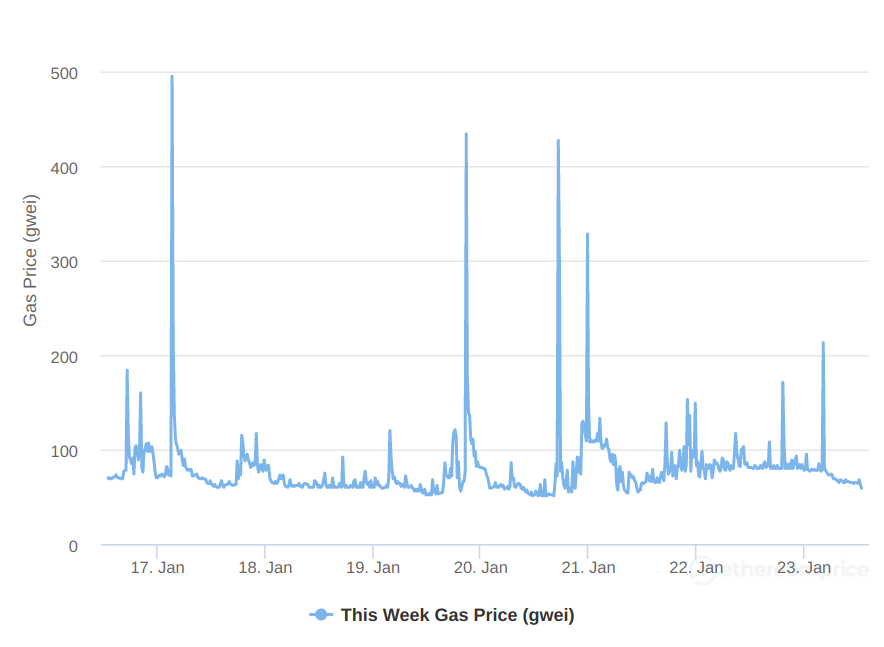
\includegraphics[width=0.9\columnwidth]{figures/ethgasprice}
    \caption
    [Price for a single gas for the week of \formatdate{17}{01}{2022}]
    {Price in gwei($10^{-8}$ ether) for a single gas for the week of \formatdate{17}{01}{2022},
        from~\cite{eth23janGasPrice}}
    \label{fig:eth-gas-price}
\end{figure}


\section{Zero-Knowledge Proofs}\label{sec:zero-knowledge-proofs}

An \textit{Interactive Proof} is a protocol where a verifier $V$ either \textit{accepts} or \textit{rejects} whether a
prover $P$ knows something~\cite{damgaard1998zk_protocols}.
For example, $P$ could be trying to convince $V$ that they know the preimage of a hash.

An interactive proof system has two key properties~\cite{smart2016zeroknowledgeproofs}:
\begin{description}
    \item[Completeness] If $P$ knows the thing being proved and follows the protocol, then $V$ should accept with
    probability one.
    \item[Soundness] If $P$ does not know the thing being proved, then $V$ should only have a negligible probability of
    accepting.
\end{description}

A \textit{Zero-Knowledge Proof} is an interactive proof with the additional property of \textit{zero-knowledge}, where
$V$ accepts without having learned any new information during their exchange with $P$~\cite{damgaard1998zk_protocols,
    smart2016zeroknowledgeproofs}.
In our example, a zero-knowledge proof where $P$ convinces $V$ that they know the preimage of a hash would require $P$
not sharing any information about (or related to) the preimage itself.

This protocol has the interesting property that the information $P$ has proven to know is still private to $V$, and
$V$ is unable to reproduce the proof and convince a third party (say, $V'$) that they (or $P$) know that information.

\subsection[zkSNARKs]{Zero-Knowledge Succinct Arguments of Knowledge (zkSNARKs)}\label{subsec:zksnarks}

% TODO do I need to go through eliptic curve math :c

Interactive proofs assume the prover is computationally unbounded (and so worries about computationally
unbounded adversaries), but by relaxing the soundness property to computationally sound proofs we can assume a
polynomial time prover~\cite{damgaard1998zk_protocols}.

This variation of an interactive proof is called an \textit{interactive argument} (because an unbounded adversary would
be able to fool $V$)~\cite{smart2016zeroknowledgeproofs}.

If we also preserve the zero-knowledge property, we have a \textit{zero-knowledge argument}, which can now be
efficient because it can run in polynomial time~\cite{naranker2022zeroknowledge}.

Additionally, if the prover is unable to construct a proof without some sort of secret (in our previous example, the
preimage of a hash function), then we have an argument \textit{of knowledge}.
Intuitively, in a zero-knowledge argument of knowledge, $V$ becomes convinced that $P$ knows some secret without the
protocol leaking any information about the secret.\\

If our zero-knowledge argument of knowledge additionally satisfies the properties of being \textit{non-interactive}~(no
or little interaction between prover and verifier) and \textit{succinct}~(the sizes of the messages are small in
comparison to the length of the actual computation), then we have a \textit{Zero-Knowledge Succinct Argument of
Knowledge} (or \textit{zkSNARK})~\cite{reitwiessner2016zksnarks}.

\subsection{zkSNARKs on Blockchains}\label{subsec:onchain-snarks}

Recent applications of zkSNARKs include privacy preserving blockchains (see~\ref{sec:bitcoin}) where a network can
verify a participant does not spend more funds that their balance without leaking any knowledge about the amount being
spent, the balance itself, or the identities of payer and payee~\cite{zerocash_whitepaper}.\\

Complex smart contracts (see~\ref{sec:ethereum}) quickly result in high costs for callers due to gas costs that increase with complexity of the
contract's computation (see~\nameref{subsec:eth:gas}).
zkSNARKs allow to verify a computation for a fraction of the cost of running it~\cite{zokrates_intro}.

% TODO cite other frameworks?
Several frameworks allow writing zkSNARKs and deploying them to a blockchain that supports smart contracts.\\

\textit{ZoKrates}~\cite{zokrates_repo} allows writing off-chain programs (which can be run tested locally) for a
verifier.
The programs can also be exported as Solidity programs~(see~\ref{subsec:eth:contract_langs})~\cite{solidity_repo} which
can then be deployed to the Ethereum network.
%TODO zokrates 1.6m gas ouch


\section{Licensing}\label{sec:licensing}

A legal agreement is a fairly broad definition which varies with each country's legal system.
Most generally, it involves~\cite{contractDef2018precedent}:
\begin{itemize}
    \item An offer by a party
    \item An acceptance by another party
    \item Intention to create a legal relationship
    \item Consideration for the offer - a sort of `promise' where a price is paid for the offer (monetary or
    otherwise).
\end{itemize}

A licence is a specific kind of legal agreement which allows a party to perform an activity under some specific
conditions\cite{licenseDefinition}.
In order to limit the scope, this project will only consider licences (rather than legal agreements as a whole).

\subsection{Dataset Licensing}\label{subsec:licensing:dataset}
See~\cite{seismicDataLicence} for an example of a licence allowing access to data by a library.
The licence includes the following clauses, cherry-picked and simplified here for clarity:
\begin{itemize}
    \item The licence is non transferable.
    \item The data cannot be sold or used to provide a service
    \item The licensee can provide access to the data to third parties provided they sign a confidentiality agreement.
    The licensee becomes liable for any breach of the licence by such third party, so it is in the licencee's interests
    that the third party also complies to the licence.
    \item The data cannot be copied or modified for any other use other than the licensee's.
\end{itemize}

See a licence by The Economist Group~\cite[\textsection2.1]{economistIU2016licence} for an example
where a clause enforces confidentiality of the terms of the agreement, not just of the data
being shared.

\subsection{Software Licensing}\label{subsec:licensing:software}
See~\cite{jetbrainsEduLicence} for an example of a software licence between a software company (JetBrains) and users for
the use of their development software.
The licence includes the following clauses, cherry-picked and simplified here for clarity:
\begin{itemize}
    \item The licence is non-transferable.
    \item The software must be used only for specific but vague purposes \textcite[for non-commercial, educational purposes
    only]{jetbrainsEduLicence}.
    \item Only the licensee may use the software, but they may install it in multiple machines simultaneously.
    \item The software cannot be sold, rented, or modified.
    \item The licensee may provide feedback - if they choose to do they themselves grant JetBrains a very permissive
    licence to use it.
    \item There is a number of exceptions where JetBrains can revoke access - but in general, they may at any point
    terminate the agreement without a specific reason.
    \item The user may choose to use an early access development version of the software, subject ot its own separate
    licence.
\end{itemize}

While this contract is not machine-readable, JetBrains does have mechanisms in place to enforce its interests.
Their software comes with a launcher, \textit{JetBrains Toolbox}~\cite{jetbrainsToolbox} that controls access to it
depending on the licence status of the user.
This is most likely implemented in a centralised server controlled by JetBrains where it keeps records
of their licensees.

For a licensee, this means they cannot easily prove they did enter an agreement with JetBrains if JetBrains chooses
to deny issuing a licence~\citeTODO.


\section{Previous Work on Machine-Readable Contracts}\label{sec:machine-readable-contracts}

In the context of this project, \emph{machine-readable}~\cite{cambridgeMachineReadable, openDataMachineReadable} refers to an encoding for a formalisation of a legal agreement which can be processed by a suitable program.
The processing must relate specifically to uses of legal documents (therefore formats like Microsoft Word, plain UTF encoded text, or PDF do not qualify).\\

See also~\autoref{sec:nlp} for normative rule generation from legal text, and~\autoref{subsec:reasoning-with-legal-agreements} for reasoning with existing formalisms.

\subsection{Juro}\label{subsec:juro}
Juro~\cite{juroWhitepaper} is a start-up business seeking to make structured machine-readable data out of contracts.
It focuses on:
\begin{itemize}
    \item Enabling easy collaboration between contract authors.
    \item Auditing and keeping track of the \textit{workflow} of the agreement (version control of the documents'
    drafts, signatures, amendments, views, etc.)
    \item Improving the user experience of employees involved in legal agreements by integrating into the company's CRM
    \textit{(Customer Relationship Management)} software (such as new hires and the Human Resources department).
    \item Ease of use by making legal documents searchable.
\end{itemize}

Juro aims to achieve this by encoding the contract as a JSON document~\cite{jsonSpec}, written by end-users
with the assistance of a web graphical user interface (GUI).
This document keeps all version control information and can be rendered into a human-readable format or exported
to PDF~\cite{pdf2020spec} or Microsoft Word~\cite{microsoftWordWeb} formats.
The JSON document can be further processed to provide extra analytics and tools, like summarization statistics or
agreement renewal reminders.\\

Juro's whitepaper lists `self-executing' clauses as future work~\cite[p.~6]{juroWhitepaper}.
Therefore Juro does not attempt to make any contributions with respect to verification of compliance or enforcement of
contract clauses.

\subsection{The Accord Project}\label{subsec:accord}

The Accord Project~\cite{accordHomepage} is an open source Linux Foundation project with the aim of enabling
machine-readable and machine-executable legal agreements.

Contracts are written pre-signature in a human-readable markup language similar to Markdown~\cite{markdownSpec}
where typed variables can be embedded.
During drafting, functions can be defined with a Domain Specific Language (DSL) that allow to perform
computations~(such as compounding interest over a period of time).

After signature, more behaviour can be written in code to check information against a contract (like checking for
breach of contract, or what action to take in a specific situation).
See Figure~\ref{fig:accord-post-signature-code} for an example where the clause checks for the state of a
delivery~(whether it is timely, has passed inspection, etc).\\

\begin{figure}[th]
    \centering
    \small
    \begin{verbatim}
    contract SupplyAgreement over SupplyAgreementModel {
      clause acceptanceofdelivery(request : InspectDeliverable) : Response {

        let received = request.deliverableReceivedAt;
        enforce isBefore(received,now()) else
          throw ErgoErrorResponse{
            message : "Transaction time is before the deliverable date."
          }
        ;

        let status =
          if isAfter(now(),
            addDuration(
                received,
                Duration{ amount: contract.businessDays, unit: days}
            )
          )
          then OUTSIDE_INSPECTION_PERIOD
          else if request.inspectionPassed
          then PASSED_TESTING
          else FAILED_TESTING
        ;
        return Response{
          status : status,
          shipper : contract.shipper,
          receiver : contract.receiver
        }
      }
    }
    \end{verbatim}
    \caption[Accord contract clause as code]{A contract clause encoded in Accord's \textit{Ergo} language,
        from~\cite{accordAfterSignatureCode}.}
    \label{fig:accord-post-signature-code}
\end{figure}

\textit{Ergo} code (the language in which Accord allows specifying contract behaviour~\cite{accordErgo}) can then be
deployed to a permissioned open-source enterprise-oriented blockchain called \textit{HyperLedger
Fabric}~\cite{hyperledgerFabric_repo, accordFabricDeployDocs} or to a NodeJS server~\cite{accordNodeJSDeployDocs}.\\

While the Accord project does also aim to represent machine-readable contracts, its representation
cannot be easily written by a non-software developer (unlike Juro's~\ref{subsec:juro}).

\subsection{Proof of Existence}\label{subsec:proof-of-existence}

Among other contributions that ease the process (not unlike Juro~\ref{subsec:juro}) of negotiating
and drafting a contract,~\cite[Express Agreement]{expressAgreement} implemented Proof of Existence,
where parties put a hash of a signed copy of a contract in the Bitcoin blockchain~(see~\ref{sec:bitcoin}).

This allows irrevocable proof of agreement verifiable by third parties.

\subsection{Ricardian Contracts}\label{subsec:ricardian-contracts}

First introduced by~\cite{grigg2004ricardian, ricardianWeb}, Ricardian Contracts aim to encode a legal agreement as a human-readable document (handwritten legal prose) accompanied by machine-readable metadata.
Additionally, it is cryptographically signed (see~\ref{fig:pubkey-signing}) by parties and uniquely identifiable;
giving it some extra cryptographic guarantees (for example, signatures cannot be plausibly denied and terms cannot be tampered with after signing).


\begin{definition}[Ricardian Contract]
    \label{def:ricardian}
    A Ricardian contract can be defined as a document that is~\cite[\textsection3.1]{grigg2004ricardian}:
    \begin{itemize}
        \item a contract offered by an issuer to holders,
        \item for a valuable right held by holders
        \item such valuable right is managed by the issuer,
        \item human-written,
        \item readable by programs,
        \item digitally signed,
        \item carrying public keys (necessary to verify signatures),
        \item uniquely identifiable through a hash digest.
    \end{itemize}
\end{definition}

Using human-written legal prose has the advantages of leading to faster dispute resolution, better enforceability and more transparency when operating within the classical framework of agreements -- for all purposes, there is no difference between a traditional agreement and a Ricardian contract in this area.\\

\subsubsection{Drawbacks}

While Ricardian contracts can represent any type of agreement, they do not actually try to capture the \emph{meaning} of a specific type of agreement.

For example, a Ricardian contract may capture all the necessary information related to a Tenancy Agreement in a format that may allow a machine to enquire about the monthly rent -- but such a machine would need to know how tenancy agreements are structured.
In short, Ricardian contracts must follow a template and it is instances of this template that are easily read and queried by machines.\\

\subsubsection{Confis as a type of Ricardian Contract}

For this one to be a successful project, it should be able to capture the meaning of an agreement it encloses.
For example, a party could be able to query about their compliance with the contract without needing to know whether the contract is a tenancy agreement, a bond, or a license.

% TODO this probably deserves its own section on how Confis tries to generalise Ricardian contracts

This project is a generalisation of Ricardian contracts in that they meet all the requirements given by definition~\autoref{def:ricardian}, but it also tries to convey and capture the meaning of the contract, so that both a machine and a human can take every single possible state into account.

Another crucial difference from what is described in~\cite{grigg2004ricardian} is that Confis does not intend to let a user write legal prose.
Rather, it hopes to produce machine-generated but human-readable prose legal prose from its internal encoding of the agreement.

\subsection{Reasoning with Legal Agreements}\label{subsec:reasoning-with-legal-agreements}

The process of representing or acquiring knowledge from a legal agreement is typically considered as a process of writing conditional rules with the following basic conditional structure~\cite{sartorLegalReasoning, ferraroLegalNLPSSurvey}:

\begin{equation}
    \label{eq:basic-rule}
    r: \text{IF} \  a_{1}, \dots ,a_n \ \text{THEN} \ c
\end{equation}

Where $r$ is the unique identifier of the rule, $a_1, \dots, a_n $ are the \emph{antecedent} representing the conditions (which includes the context under which the rule is created) of applicability of the norm, and $c$ is the \emph{conclusion} representing the effect of the norm.\\

Note how~\nameref{subsec:juro} does not try to capture norms at all, and~\nameref{subsec:accord} chooses to use the abstraction of a program rather than that of a set of rules.
NLP, on the other hand (discussed in~\autoref{sec:nlp}) struggles to extract such rules from existing documents.

\subsubsection{Contract-Driven Agents}\label{subsubsec:contract-driven-agents}

An attempt at formalising a representation of the behaviours involved in a legal agreement and the interactions between the parties to such agreements contract-driven agents as presented in~\cite{knottenbeltContractDriven}.\\

The formalisation involves establishing a calculus based in multi-agents systems specifically oriented towards legal agreements, through the event calculus as first introduced by~\cite{kowalski1989logicEventBased}~(a logic-based system).
Note how the event calculus can be generalised by~\autoref{eq:basic-rule}.\\

Unlike Ricardian contracts~(see~\autoref{subsec:ricardian-contracts}), contract-driven agents attempt to describe the behaviours of all parties as well as how they react to other parties' behaviours.
Therefore, unlike Ricardian contracts, they also capture the semantics of the agreement between the contract.


\subsubsection{Symboleo}

TODO talk about~\cite{symboleo2020}


\section{Natural Language Processing and its Limitations}\label{sec:nlp}

Human-written text, which is how legal agreements are typically persisted\footnote{Note other formats like verbal agreements may also constitute legal agreements~\cite{larsonContractLawIntro}} can be converted into machine-readable form by attempting to translate the natural language in which they are written through Natural Language Processing~(NLP), which uses techniques such as symbolic reasoning and deep learning~\cite{GoldbergNLPReview}.\\

Existing technologies trying to process legal text -- such as~\cite{angeli2015NLP1},~\cite{lapata2016NLP2},~\cite{lapata2018NLP3}, or~\cite{sleimi2018NLP4} -- try to produce normative rules.

At the time of writing, they fall short of fully capturing all relevant information in an existing legal document -- therefore they lack the~\nameref{def:completeness} property discussed in~\autoref{sec:eval:goals}.
They face the main following challenges~\cite{ferraroLegalNLPSSurvey}:

\paragraph{Cross-referencing}

Legal text is structured into sections and subsections which contain sentences which represent clauses applicable in a specific context.
Documents therefore often reference information across sections or across documents.
Some of these references may not even be explicit: often, contracts have a `Definitions' section solely for the role of disambiguating terms which the reader is expected to use in their understanding of the document.

NLP solutions must therefore be able to deal with referencing in order to extract context and resolve lexical ambiguities.

\paragraph{Ambiguity}
While legal documents aim to remove ambiguity and ideally produce a single interpretation, unintended ambiguities arise from the use of natural language.

The most likely ambiguity is \emph{referential ambiguity} where a word or phrase has multiple meanings inferred from current context, from a parent statement (which is unique to legal text), or from other document sections via cross-referencing.

Natural language can also represent different logical interpretations, which is referred to as \emph{local ambiguity}.
An example of this is using the term ``and'' to represent a disjunction instead of a conjunction.

\paragraph{Sentence Complexity}

Sentences used in legal prose tend to be much longer than sentences from other domains.
The average number of lexical units in a sentence written in English in Wikipedia is about 19~\cite{wiki19words}, while sentences from a legal document can have more than 50~\cite{ferraroLegalNLPSSurvey} as well as have complex syntactic structures (see for example~\autoref{fig:geophys-long-clause}).

Current NLP technologies struggle with such sentences: syntactic analysers and predicate-argument extraction tools sometimes do no correctly capture the scope of coordinate conjunctions, nor the antecedents of subordinate phrases.

\begin{figure}[h]
    \centering
    \fbox{
        \begin{minipage}{0.8\textwidth}
            On termination of this Licence the Licensee shall cease to have any rights or Licence in
            respect of the Data or any adaptation thereof and shall cease to use the same and shall
            erase the Data or any adaptation thereof from any storage apparatus and shall return to
            the Library without demand the Data and all existing copies thereof made by the
            Licensee and shall warrant in writing to the Library that all data, plots, displays, results,
            analyses, variations and modifications derived from the Data are destroyed.
        \end{minipage}
    }
    \caption{Clause \textsection3.2 of~\citetitle{seismicDataLicence}~\cite{seismicDataLicence}}
    \label{fig:geophys-long-clause}
\end{figure}

\paragraph{Normative Effects and Modalities}

Legal documents typically encode norms, and words specific to legal concepts such as \emph{right, power, immunity, liability, privilege}, etc significantly alter the way a sentence is interpreted.
Properly capturing modalities or behaviours such as a \emph{requirement} or a \emph{permission} is a major difficulty the state of the art of Artificial Intelligence in Law struggles to deal with~\cite{ferraroLegalNLPSSurvey}.


\section{Domain-Specific Languages}\label{sec:dsls}

The use-case of representing complex, formalised abstractions in a machine-readable formats is a common one, and general-purpose programming languages (Java, Python, etc) are designed with exactly this goal in mind.

A class of languages made to target a specific problem, rather than being general purpose, also exists: these are \emph{Domain-Specific Languages} (or \emph{DSLs})

According to~\cite{fowlerDsl}: ``A DSL is a computer language that is targeted to a particular kind of problem, rather than a general purpose language that is aimed at any kind of software problem''.
In order to write legal agreements and lower the barrier of entry as much as possible (ideally, no software engineering training should be required) a well-documented and easy-to-use DSL is a good solution: expressive enough to be able to represent a large range of agreements, but restrictive enough that language features should not require extensive training.\\

Several modalities of DSLs exist that can be used.
The compromises they make are in cost (for developing a framework for them), ease of writing, readability, and expressiveness~\cite{fowlerDslGuide, fowlerLangWorkbench}.

\paragraph{Textual Internal DSLs}

Textual Internal DSLs make use of a host language, and use that language constructs in particular ways to give the internal DSL a particular feel.
They share their syntax with and are a subset of their host language.
This solution is the easiest to develop but forces the DSL author to conform to a host language and to extend their DSL within the bounds of what the host language can do.

\paragraph{Textual External DSLs}

Textual External DSLs have their own custom syntax and therefore they need a full new parsed to be processed.
This solution provides the most flexibility in what the language can express but is more expensive in terms of development efforts for the DSL author.

\paragraph{Graphical DSLs}

While Textual DSLs require writing and parsing text, graphical DSLs can be achieved with a tool providing a graphical user interface that then builds some internal representation that can be processed.
This solution is the most accessible for users of the DSL with non-technical backgrounds but is also expensive in terms of development cost, as both an internal representation and a GUI builder must be developed.

% TODO revisit figure placement in this section :c

\subsection{Candidates for Internal DSL Host Languages}\label{subsec:dsl-host-candidates}

This project is concerned with making a DSL with low development costs, and as such it will consider several platforms as host language candidates for an internal DSL\@.
\begin{definition}[DSL Host Traits]
    \label{def:host-lang-requirements}
    Languages desirable to be host for DSLs usually have some of the following features:
    \begin{itemize}
        \item \textbf{Operator overloading} for easily including symbols familiar to most users in the language, such as \texttt{`+'}, \texttt{`-'}, \texttt{`\&'}, etc.
        \item \textbf{Infix functions} for constructing sentence-like expressions or statements, such as \texttt{`if car is parked'}.
        \item \textbf{Scripting facilities} that allow compiling a small text snipped without having to define a full program that includes an entrypoint.
        \item \textbf{A Tooling Platform} which allows developing tools which enahnce the wiritng experience.
        Examples of this include GUI builders and IDE features (like syntax highlighting and inline compiler warnings).
        \item \textbf{Scripting}~(see~\autoref{subsec:scripting-support}) which allows parsing stand-alone text files in the host language that are interpreted by a DSL-aware host.
    \end{itemize}

\end{definition}

\subsubsection{Haskell}

Haskell~\cite{haskellDocs} is a functional programming language which can be compiled or interpreted.
It has advanced features including most of the ones mentioned in~\nameref{def:host-lang-requirements}.

These are demonstrated in~\autoref{fig:haskellBasicDsl}, where Haskell functions are used as commands and statements of the BASIC language.
This results in a valid Haskell expression (with some language modifications) that also defines a valid BASIC program -- therefore allowing to write and compile BASIC without actually needing a BASIC parser.

\begin{figure}[h]
    \centering
    \begin{minipage}{0.8\textwidth}
        \begin{minted}[
            autogobble,
            frame=lines,
            framesep=2mm]{haskell}
    {-# LANGUAGE ExtendedDefaultRules, OverloadedStrings #-}
    import BASIC

    main = runBASIC $ do
        10 GOSUB 1000
        20 PRINT "* Welcome to HiLo *"
        30 GOSUB 1000

        100 LET I := INT(100 * RND(0))
        200 PRINT "Guess my number:"
        210 INPUT X
        220 LET S := SGN(I-X)
        230 IF S <> 0 THEN 300

        240 FOR X := 1 TO 5
        250   PRINT X*X;" You won!"
        260 NEXT X
        270 STOP

        300 IF S <> 1 THEN 400
        310 PRINT "Your guess ";X;" is too low."
        320 GOTO 200

        400 PRINT "Your guess ";X;" is too high."
        410 GOTO 200

        1000 PRINT "*******************"
        1010 RETURN

        9999 END
        \end{minted}
    \end{minipage}
    \caption[BASIC program written in a Haskell DSL]
    {A BASIC program written in a Haskell DSL, from~\cite{haskellBasicDSL}}
    \label{fig:haskellBasicDsl}
\end{figure}

Haskell additionally permits defining the precedence of operators and infix functions, allowing to define the direction in which associativity propagates~\cite{haskellFixity}.
This can be useful to form English-like sentences in a DSL such as \texttt{`Bob did eat after Alice did eat'}, where \texttt{`after'} can be an infix function with lower precedence that \texttt{`did'}, which forms the other two sentences.

\paragraph{Tooling} Haskell tooling is comparatively lacking next to more mainstream general purpose programming languages (such as Kotlin) in that the communities developing its tooling platform are smaller.

\subsubsection{Groovy}

Groovy~\cite{groovyLangIndex} is a general purpose language with plenty of features specifically designed for DSLs.
One of the most used examples of such DSLs is the Gradle Build Language~\cite{gradleDSL} which specifies configuration for the Gradle build tool.
This sets the build tool apart from similar tools, like Maven and Makefiles, which do not use DSLs.
An example of a script for such a DSL is given in~\autoref{fig:gradleGroovyDSL}.

\begin{figure}[h]
    \centering
    \begin{minipage}{0.8\textwidth}
        \begin{minted}[
            autogobble,
            frame=lines,
            framesep=2mm]{groovy}
            plugins {
                id 'groovy'
                id 'application'
            }

            repositories {
                mavenCentral()
            }

            dependencies {
                implementation 'org.codehaus.groovy:groovy-all:3.0.9'
                implementation 'com.google.guava:guava:30.1.1-jre'

                testImplementation 'junit:junit:4.13.2'
            }

            application {
                mainClass = 'demo.App'
            }

            tasks.named('test') {
                useJUnitPlatform()
            }
        \end{minted}
    \end{minipage}
    \caption[Gradle Groovy Build script]
    {A Gradle Groovy build script, from~\cite{gradleDSL}}
    \label{fig:gradleGroovyDSL}
\end{figure}

Unlike to the other candidates in this section, Groovy allows for dynamic typing.
This means that the language offers more runtime flexibility when designing a DSL, as new variables and classes can be created as the script is interpreted.

\paragraph{Tooling} Groovy has feature-rich tooling that allows parsing standalone scripts with a DSL context, but its external tooling (like intelligent editors) is limited due to the nature of its runtime dynamic typing.
In the example of~\autoref{fig:gradleGroovyDSL}, an editor would not be able to suggest autocompletion for \texttt{`useJUnitPlatform()'} inside the configuration of the \texttt{test} task.

\subsubsection{Kotlin}\label{subsubsec:kotlinLang}

Kotlin~\cite{kotlinLang} is another general-purpose language.
The language supports infix functions and operator overloading.
An example DSL that uses Kotlin as the host language is given in~\autoref{fig:kotlinHtmlDsl}.

\begin{figure}[h]
    \centering
    \begin{minipage}{0.9\textwidth}
        \begin{minted}[
            autogobble,
            frame=lines,
            framesep=2mm]{kotlin}
        fun main(args: Array<String>) {
            val generated = html {
                head {
                    title {+"XML encoding with Kotlin"}
                }
                body {
                    h1 {+"XML encoding with Kotlin"}
                    p  {+"this can be used as an alternative to XML"}

                    // an element with attributes and text content
                    a(href = "https://kotlinlang.org") {+"Kotlin"}

                    // content generated by
                    p {
                        for (arg in args)
                            +arg
                    }
                }
            }
            println(generated.toString())
        }
        \end{minted}
    \end{minipage}
    \caption{Kotlin DSL for building HTML, from~\cite{kotlinTypeSafeBuilders}}
    \label{fig:kotlinHtmlDsl}
\end{figure}

\paragraph{Tooling} While the language is not as flexible as Haskell or Groovy, it is supported by well-maintained and feature-rich external tooling (in terms of the \textit{IntelliJ IDEA} editor) and has stand-alone scripting support~\autoref{subsec:scripting-support}.

% TODO add link on why we used this
Additionally, the editor IntelliJ IDEA supports live evaluation of Kotlin inside text boxes, allowing to provide hints at the same time it compiles a specific snippet of code~\cite{intelliJRepo}.

\subsection{Scripting Support}\label{subsec:scripting-support}

Depending on the DSL being developed, it may be necessary for the host language to provide scripting support.
By \emph{scripting support}, we mean allowing a program to evaluate a file or a string of text, at runtime, and share properties with the file.
We will call this file a \emph{script}.

In general, interpreted languages offer this functionality through \texttt{`eval(...)'} methods or similar.
They may not be necessarily well-suited for a DSL as they also tend to have weak or dynamic typing (this is the case of Python, for example).
Other compiled languages may offer this functionality:
\begin{itemize}
    \item Java offers it through JSR 223~\cite{javaScripting} and allows languages other than Java in the scripts.
    \item Kotlin~\cite{kotlinScriptKeep}.
    \item Groovy~\cite{groovyScripting}, which is widely used inside the Gradle build system (see~\autoref{fig:gradleGroovyDSL} for an example) where Gradle DSL scripts make up the configuration build files (in a way comparable to Makefiles).
\end{itemize}

For DSLs in particular, there is the requirement that the scripting host is aware of the DSL when evaluating the script~\cite{kotlinScriptKeep}.
This is what allows using a library-defined function in a stand-alone file without compiling errors.
Notice how this is not the case of the Haskell and Kotlin DSL examples in~\autoref{fig:haskellBasicDsl} and~\autoref{fig:kotlinHtmlDsl} (where imports and program entry-points are necessary).
% TODO section on the main differences between machine-readable representations of contracts?


\section{Language Tooling}\label{sec:language-tooling}

Most Integrated Development Environments (or IDEs) have support for \emph{extensions} or \emph{plugins} that allow extending their functionality~\cite{ideaExtensionPoints, vscodeExtensions}.
A common use-case for this is enhancing developer productivity by providing visual cues and aids to textual development by, for example, reporting compilation errors and warnings inside an editor.

Extensions also typically allow arbitrary graphical user interfaces inside the program window, with access to the contents of the files opened.

\subsection{Custom Scripting Support in IntelliJ IDEA}\label{subsec:scripting-in-intellij}

The IntelliJ IDEA editor~\cite{intelliJRepo} allows a specific extension point for providing script definitions~\cite{kotlinScriptKeep, ideaExtensionPoints} and enabling development features such as syntax highlighting, error reporting, and autocompletion inside custom-defined scripts.

